% Extracted without edits from the BA-clarified SI's Figure S15.
\documentclass[tikz,border=3pt]{standalone}
\usepackage[T1]{fontenc}
\usepackage{lmodern,amsmath,amssymb}
\usetikzlibrary{arrows.meta,calc}
\begin{document}
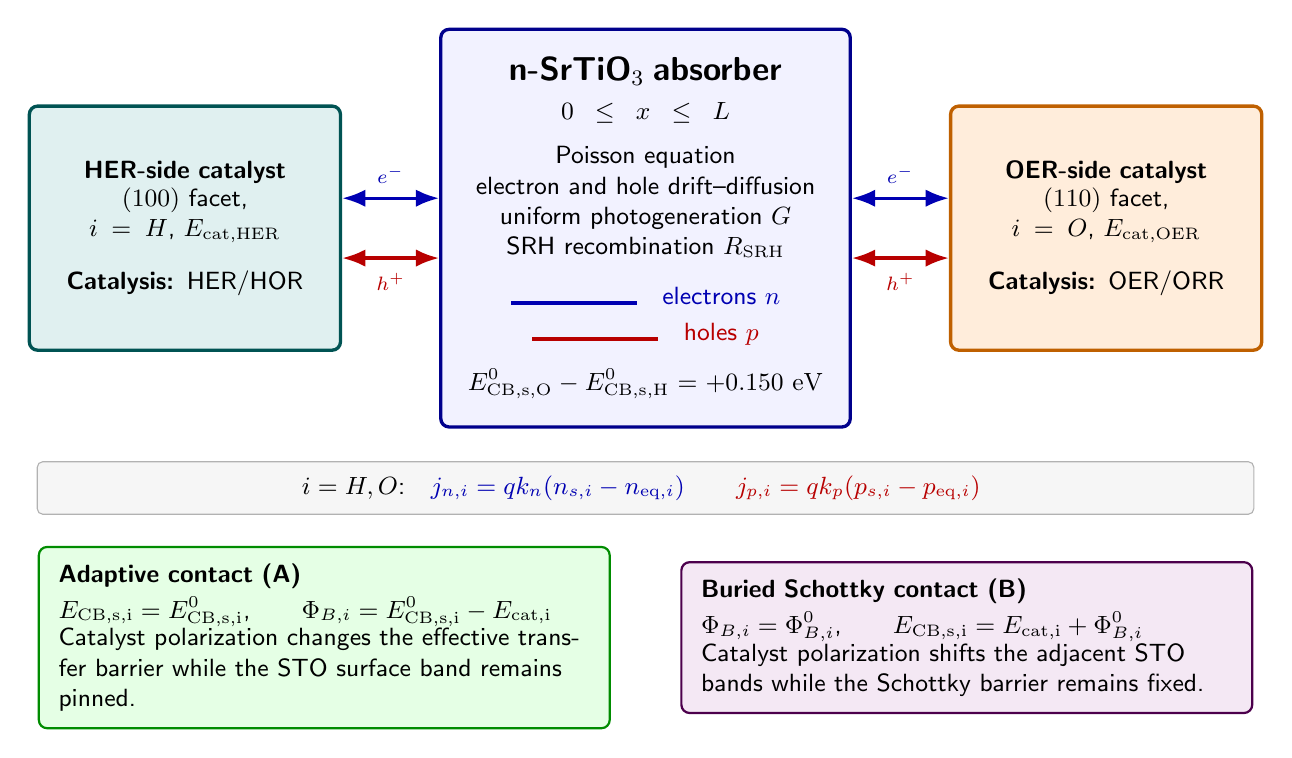
\begin{tikzpicture}[
  x=1cm,y=1cm,
  font=\small\sffamily,
  >=Latex,
  contact/.style={draw,very thick,rounded corners=3pt,align=center,inner sep=5pt},
  transfer/.style={<->,very thick},
  condition/.style={draw,thick,rounded corners=3pt,align=left,inner sep=6pt}
]
\node[contact,fill=teal!12,draw=teal!65!black,minimum width=3.95cm,
      minimum height=3.10cm,text width=3.60cm] (her) at (2.05,6.35) {%
  \textbf{HER-side catalyst}\\[-1pt]
  $(100)$ facet, $i=H$, $E_{\rm cat,HER}$\\[8pt]
  \textbf{Catalysis:} HER/HOR
};

\node[contact,fill=blue!5,draw=blue!55!black,minimum width=5.20cm,
      minimum height=5.05cm,text width=4.70cm] (sto) at (7.90,6.35) {%
  {\large\textbf{\emph{n}-SrTiO$_3$ absorber}}\\[3pt]
  $0\leq x\leq L$\\[5pt]
  Poisson equation\\
  electron and hole drift--diffusion\\
  uniform photogeneration $G$\\
  SRH recombination $R_{\rm SRH}$\\[7pt]
  \textcolor{blue!70!black}{\rule{1.6cm}{1.2pt}\quad electrons $n$}\\[2pt]
  \textcolor{red!72!black}{\rule{1.6cm}{1.2pt}\quad holes $p$}\\[7pt]
  $E_{\rm CB,s,O}^{0}-E_{\rm CB,s,H}^{0}=+0.150~\mathrm{eV}$
};

\node[contact,fill=orange!14,draw=orange!75!black,minimum width=3.95cm,
      minimum height=3.10cm,text width=3.60cm] (oer) at (13.75,6.35) {%
  \textbf{OER-side catalyst}\\[-1pt]
  $(110)$ facet, $i=O$, $E_{\rm cat,OER}$\\[8pt]
  \textbf{Catalysis:} OER/ORR
};

\draw[transfer,blue!70!black] ([yshift=0.38cm]sto.west) -- ([yshift=0.38cm]her.east);
\draw[transfer,red!72!black]  ([yshift=-0.38cm]sto.west) -- ([yshift=-0.38cm]her.east);
\draw[transfer,blue!70!black] ([yshift=0.38cm]sto.east) -- ([yshift=0.38cm]oer.west);
\draw[transfer,red!72!black]  ([yshift=-0.38cm]sto.east) -- ([yshift=-0.38cm]oer.west);

\node[fill=white,inner sep=1pt,font=\scriptsize\bfseries,text=blue!70!black]
  at ($(her.east)!0.5!(sto.west)+(0,0.68)$) {$e^-$};
\node[fill=white,inner sep=1pt,font=\scriptsize\bfseries,text=red!72!black]
  at ($(her.east)!0.5!(sto.west)+(0,-0.68)$) {$h^+$};
\node[fill=white,inner sep=1pt,font=\scriptsize\bfseries,text=blue!70!black]
  at ($(sto.east)!0.5!(oer.west)+(0,0.68)$) {$e^-$};
\node[fill=white,inner sep=1pt,font=\scriptsize\bfseries,text=red!72!black]
  at ($(sto.east)!0.5!(oer.west)+(0,-0.68)$) {$h^+$};

\node[draw=gray!60,fill=gray!7,rounded corners=2pt,align=center,
      minimum width=15.45cm,inner sep=5pt] at (7.90,3.05) {%
  $i=H,O$:\quad
  \textcolor{blue!70!black}{$j_{n,i}=qk_n(n_{s,i}-n_{{\rm eq},i})$}\qquad
  \textcolor{red!72!black}{$j_{p,i}=qk_p(p_{s,i}-p_{{\rm eq},i})$}
};

\node[condition,fill=green!10,draw=green!55!black,minimum width=7.25cm,
      text width=6.75cm] at (3.82,1.15) {%
  \textbf{Adaptive contact (A)}\\[2pt]
  $E_{\rm CB,s,i}=E_{\rm CB,s,i}^{0}$,\qquad
  $\Phi_{B,i}=E_{\rm CB,s,i}^{0}-E_{\rm cat,i}$\\[-1pt]
  Catalyst polarization changes the effective transfer barrier while the STO surface band remains pinned.
};
\node[condition,fill=violet!9,draw=violet!60!black,minimum width=7.25cm,
      text width=6.75cm] at (11.98,1.15) {%
  \textbf{Buried Schottky contact (B)}\\[2pt]
  $\Phi_{B,i}=\Phi_{B,i}^{0}$,\qquad
  $E_{\rm CB,s,i}=E_{\rm cat,i}+\Phi_{B,i}^{0}$\\[-1pt]
  Catalyst polarization shifts the adjacent STO bands while the Schottky barrier remains fixed.
};
\end{tikzpicture}
\end{document}
